\documentclass{scrreprt}
\usepackage{glossaries}
\usepackage{listings}
\usepackage[]{graphicx}

\newglossaryentry{latex}{
  name=LaTeX,
  description={Ein Textsatzsystem}
}
\newglossaryentry{consumer}{
    name=Consumer,
    description={A program using a UaDI conform DLL to get generated data from a producer or device}
}
\makeglossaries

\tableofcontents
\newpage 

\begin{document}

\chapter{The Idea of OmniView}
OmniView is planned to be an omniscient data-visualization and analysis tool. 
OmniView itself shouldn't need to know anything about any given data-producer at compile-time, but should still be able to visualize the produced information.
OmniView itself shouldn't need to know anything about any given analysis-tool at compile-time, but should still be able to use an analysis-API. 
In order for OmniView to work this way, there shall be a structured architectural approach, to enable modular development.
This includes dataproducer devices as well as analysis-tools.

\section[Modules]{Modules of OmniView and their Role}
The Name OmniView actually only applies to the executable instance, that is in charge of displaying gathered data in a way similar to PicoScope or sigrok, whether it's live or archived data. 
Since (well-designed) modularity can help keeping the complexity of a system in check, the greater OmniView-Architecture is a project of the Bochumer AI-Group.
\\
A oscilloscope-like user-interface is the most generic way, to display data as a function over time. 
All measurement-values are a sample of a certain unit (sometimes even an SI-Unit) at a specific point in time, and thus projectable onto a plane with its unit in y- and the time in x-dimension. 
Displaying a multitude of different y-dimensions in an oscillogram is a well-proven design and has been implemented in several data-recorder software-suites. 
\\
Incoming live-data into the view is delivered via a websocket connection.
There won't be hard real-time guarantees in this interface. 
This websocket is provided by an entity that implements the concept of an epoch-server.
Soft real-time can be guaranteed to a certain extend in the internal structure of the epoch-server and its storage-interface.
Due to the nature of live-updates of a GUI, new updates are being received on a regular basis and prepended to the n-1 dataset.
Each update-object that contains data to be prepended, and displayed in the oscillogram is called a column. 
It derives its name from the property, that it holds several values of different data-channels in parallel.
The aggregation to a continuous stream of such pieces of information that belong to one channel is called a waveform. 
\\
An epoch-server has the ability to maintain multiple websocket connections, and an OmniView-Instance has the ability to maintain connections to multiple epoch-servers. 
Before a view can instantiate a connection with a websocket, it queries the epoch-servers REST-API, to receive a structure know as possibility-list.
This list contains all available devices, and all available transducers. 
A transducer is a function that works as a filter.
It implements a directed node, taking one or more waveforms as an input and having exactly one waveform as an output. 
Using transducers, a so-called (processing-)route can be constructed. 
A route is a directed graph composed from transducer-nodes. 
For further investigation see \ref{chap:WaveformProcessingNetwork}.
The structure inside the epoch server that defines which channels are being send out to a specific connection is called the connections visibility-list. 
This list in combination with a checkbox will also be displayed in the view.

\begin{figure}
    \includegraphics[\width=.9]{assets/overview.pdf}
    \caption{Overview of Modules}
\end{figure}

\section[Greater Picture]{OmniView and its Role in the Greater Picture}
Auto-Intern GmbH and their connected entities have been working on a unified architecture for measurement- and monitoring-devices since the early 2000s. 
Integrating measurement-systems into larger architectures is by no means a trivial task.
OmniView fits into the Grand-Unified-Monitoring-Architecture of Auto-Intern.


\begin{figure}
    \includegraphics[width=.9\textwidth]{./assets/pictures/overview.pdf}
    \caption[]{Brief overview of the proposed structure}
    \label{fig:overview}
\end{figure}


There shall be a unified way to interact with an abstract data-producer.
This includes devices such as:
\begin{enumerate}
    \item a USB-oscilloscope \gls{latex}
    \item a TCP/IP client, sending a continuous stream
    \item a USB-logic-analyzer
    \item a random-number-generator
    \item a filedescriptor
\end{enumerate}

Since it is not known at compile-time, which devices will be used at runtime, the code can't be linked statically into OmniView (or any other data-\gls{consumer} for that matter). 
Therefor an interface shall be defined, that gets used by the consumer, but the implementation of the data-handling ought to be provided in a dynamically linked library. 
From here on forward we will refer to this as \lstinline|DLL| even though \lstinline|.dll| and \lstinline|.so| are meant equally. 
If a windows \lstinline|.dll| or a linux \lstinline|.so| is meant specifically, please use the terms \lstinline|.dll| or \lstinline|.so|, otherwise \lstinline|DLL|. 
Be aware, that this \lstinline|DLL| does not necessarily constitue an aquivalent to an actual device-driver with a communication-channel to the systems kernel.
\\
It appears, that all dataproducers that are relevant for OmniView can be abstracted in a certain way, and thus share the same function-calls in a \lstinline|DLL|.
There are three requirements:
\begin{itemize}
    \item Grabbing the next part of the data-stream asynchronusly
    \item The data-producer providing meta-information about itself 
    \item Send control-data from the consumer to the data-producer
\end{itemize}
This interprocess-communication comes with some additional hurdles.

\section{Memory Management Ideology}
Not only does OmniView not know about which devices will be connected at runtime, it also does neither know about the amount of devices that will be attached, nor does it know what data-rate the producers will provide.
Due to this uncertainties, a strongly structured memory allocation ideology needs to be implemented in order to minimize error-prone sections in the applications code.


\section[UaDI]{Unified abstract Data\-producer Interface}
The \textit{Unified abstract Data\-producer Interface} is the protocol that specifies the interprocess\-communication between the con\-sumer and the device, using the \lstinline|DLL|. 

\begin{figure}
    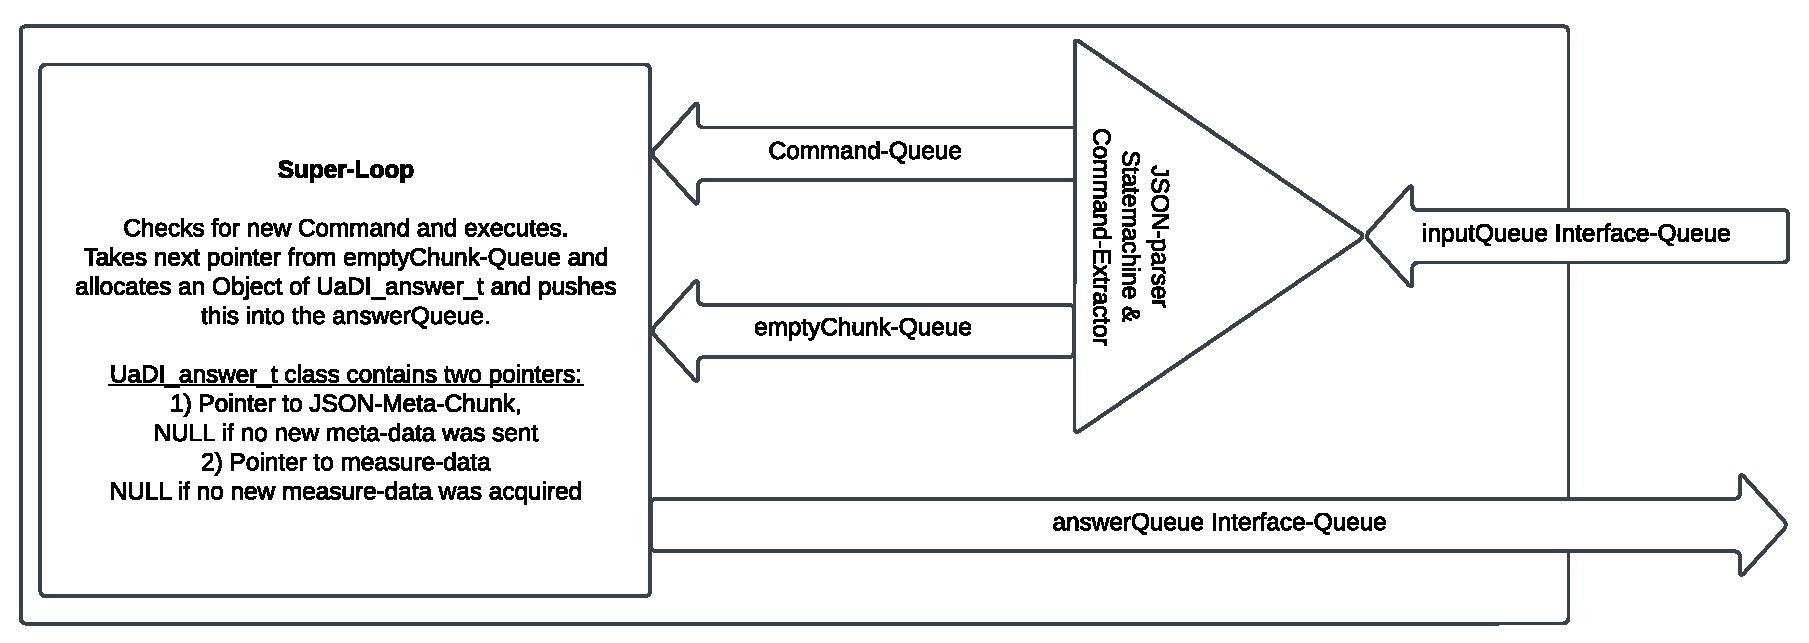
\includegraphics[width=.9\textwidth]{./assets/pictures/interface.pdf}
    \caption[]{Coarse structure of the DLL-interface}
    \label{fig:dllinterface}
\end{figure}


\chapter{Dataproducers}
The origin of a stream of measurement-samples is called a device, as refered to in the UaDI specification. 
A device may get control-input, but always has to back-channels to a consumer:
\begin{itemize}
    \item a pointer to a JSON chunk
    \item a pointer to a data chunk
\end{itemize}
\section{Memory-Management}
A device doesn't allocate on its own.
Therefor it needs to get a memory-pointer from the consumer.
The so called chunks are of a default size of 128*1024 bytes.
Pointer to these memory-locations are known as chunk\_ptr.
The consumer is responsible for the memory management of these chunks.
An array of chunk\_ptr can be handed to the device on claiming it, as well as through a routine called uadi\_push\_chunk.
In both cases, the consumer passes an array of chunk\_ptr, and the amount of chunk\_ptr to the device.
When claiming the device, a callback is also registerd. 
The callback is called, when the device is finished with writing into a chunk.
The callback is called with a chunk\_ptr and a void pointer to the consumers context. 
The device doesn't care about the context pointer, it just hands it back to the consumer.
Which data-type the device hands back is defined by the device. 
In the first usecases, only float shall be supported. 
The data-type will be handled in a second layer on top of UaDI, that performs device-management.

\section{Concrete Devices}
There are several devices already planned that need to be supported by the end of 2024:
\begin{enumerate}
    \item OmniScope - USB-Single-Channel Oscilloscope
    \item OmniScope Duo - USB-Dual-Channel Oscilloscope
    \item OmniEField - USB-E-Field Probe
    \item OmniBField - USB-B-Field Probe
    \item OmniTherm - USB-Thermocoupler Typ-K 
    \item OmniPower - USB-Power-Monitor
    \item OmniPower ETH - Ethernet-Power-Monitor
    \item OmniSonic - USB-Vibration-Sensor
    \item AI PowerProbe - Ethernet E-Field/B-Field Probe 
    \item Random Number Generator Software-Device
    \item IOTA Software Device 
    \item PCIe - Generic Integer Kintex7 FPGA Device
\end{enumerate}


\section{Userinterface}

The following paragraphs describe the Userinterface components and their functionality.
The design of individual components is also introduced here; however, the detailed description of the design principles can be found in Chapter \ref{cap:Designprinciples}. All components should be designed after those principles.\\ 

The user interface is currently implemented in C++; however, there are plans to transition it to JavaScript in a subsequent phase.\\
This interface serves as a central hub for configuring connected devices, conducting measurements, saving data in various formats, displaying and analyzing the acquired data. Additionally, users can access an integrated Help Menu that directs them to a website providing comprehensive information about OmniView and OmniScope.

The basic interface should contain 

\begin{itemize}
    \item a bar at the top where the company name, a saving button, a settings button, a start and stop measurement button are integrated 
    \item an adjustable window where the data is displayed
    \item a side menu which can be minimized for : 
    \begin{itemize}
        \item searching devices 
        \item loading old data 
        \item Diagnostics
        \item Settings
        \item Help
    \end{itemize}
    \item a bottom window which can be minimized where the connected devices and the loaded data files are presented
    \item serveral popup windows that are displayed when using for example a analyses
\end{itemize}

The design should look like the following picture. Right now all buttons are in German, which should be changeable later through the settings menu. 

The popup windows will be 
\begin{itemize}
    \item a window to upload the data
    \item a window to save the data 
    \item a window to check the old data analyses results 
\end{itemize}

This popup windows should all follow the same structure and design principles which can be found in the \ref{cap: Designprinciples}. 
An example for a popup window is shown in Figure \ref{fig:PopupwindowDesign}.
This list is not yet completed. 

% insert picture 
The detailed descriptions of the individual components and their functionality is described in the following sections.


\subsection{Toolbar}

The toolbar will be displayed at the top of the programm. 
A picture is shown in figure \ref{fig: toolbar}. 
\begin{figure}
    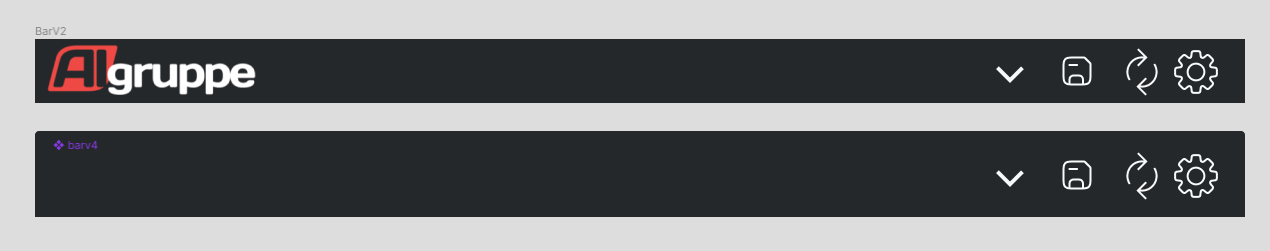
\includegraphics[width=.9\textwidth]{assets/pictures/Toolbar states.png}
    \caption[]{A visual representation of the Toolbar with different buttons}
    \label{fig:saveData}
\end{figure}
The toolbar contains the company logo at the left side, this logo should only be visible when the side menu is closed. 
At the right side the toolbar contains a save button, a settings button and a load again button. 
In the middle of the toolbar is a field for starting and stopping the measurements that has different states depending on the current state of the measurement. 

In the following the functionality of the different buttons is descriped. 

\subsubsection{Save button}

The save button should be a Icon button that follows the design principle of the icon button described in chapter \ref{cap:Designprinciples_IconButtons}. 
The save button is used to write the measurement (a waveform stack) into a storage. 
The measurement is defined as a waveoform stack because the user is able to save the measurement from only one devices or from many different devices into one or more files.

This section delineates the procedure for transferring the data from a waveform stack or an individual waveform, acquired through the OmniScope, to a storage system via the user interface. The storage options encompass the computer's file system, a Database Management System (DBMS), or a Cloud platform. Refer to \cite{fig:saveData} for a visual representation of the corresponding menus.\\

The following describes the User story: \\

Visibility of Save Button: \\

Prior to initiating the measurement, the save button should be prominently visible.\\

Greyed-out State During Measurement:\\

While the measurement is in progress, the save button should appear in a greyed-out state.\\

Post-Measurement Access:\\

Upon completion of the measurement, users should easily locate and access the now visible save button.\\

Prompt Appearance of Save Window:\\

When the user clicks the save button, a window should promptly appear. This window should be designed after the design principle in chapter \ref{cap:Designprinciples_Popupwindows}\\

Window Components:\\

Within the window, an input field labeled "Speicherpfad" should be positioned in the left corner, accompanied by a "Durchsuchen" button. The buttons should be designed after the design principle in chapter \ref{cap:Designprinciples_PopupWindowButtons}\\

Path Input Options:\\

Users have the option to manually input a path into the "Speicherpfad" field.\\

File-Explorer Integration:\\

By clicking the "Durchsuchen" button, the File Explorer opens, enabling users to manually select a saving path.\\

Default Path Handling:\\

If no path is selected, the system defaults to using Desktop/Omniview/saves/.\\

Visible Default Path:\\

The default path is displayed in the "Speicherpfad" field, appearing greyed out.\\

Device Selection:\\

Users can choose the devices for saving through a dropdown menu under the selected path.
Only the devices that are connected are shown with their correct device name.
Also files that have been loaded into the devices list are shown.
The number of connected devices is undetermined before the start of the software so their can be multiple devices or just one.\\

Adding Another Path:\\

In cases where multiple devices are connected, users can click "Add another path," triggering the appearance of another window with identical settings. Here the user also has a "Durchsuchen"-Button where he can choose in which path the data is stored and a drop down menu to choose which devices he wants to be stored in the selected path. The user can also change the name of the measurement.\\

Checkbox Selection:\\

When checkboxes next to the devices are selected, the chosen devices are saved in the same file within the selected directory.\\

Vehicle Information Input:\\

Beneath the "Speicherpfad," three input fields—Vehicle type, VIN, measurement name, and mileage—are available.\\

Dropdown Menu for Vehicle Type:\\

Users can choose the vehicle type via a dropdown menu loaded from a file.\\

Adding Custom Vehicle Type:\\

An option allows users to input a new vehicle type at the end of the dropdown menu, subsequently adding it to the file by clicking a plus button.\\

Final Save Action:\\

Users can initiate the save process by clicking the save button in the right corner, preserving the selected waveform stack in the chosen path as a .csv file. The filename should contain the name of the device and a name set by the user in the "Messung"-field.\\

Information Inclusion in File Name:\\

The information entered about the vehicle ("Messung", "vin", "bekannte Fahrzeuge") should be saved at the top of the csv. file, so it can be read out in a later process.\\
Exit Option:\\

Throughout the entire process, users can close the window by clicking an exit button located in the right corner of the window.\\


\begin{figure}
    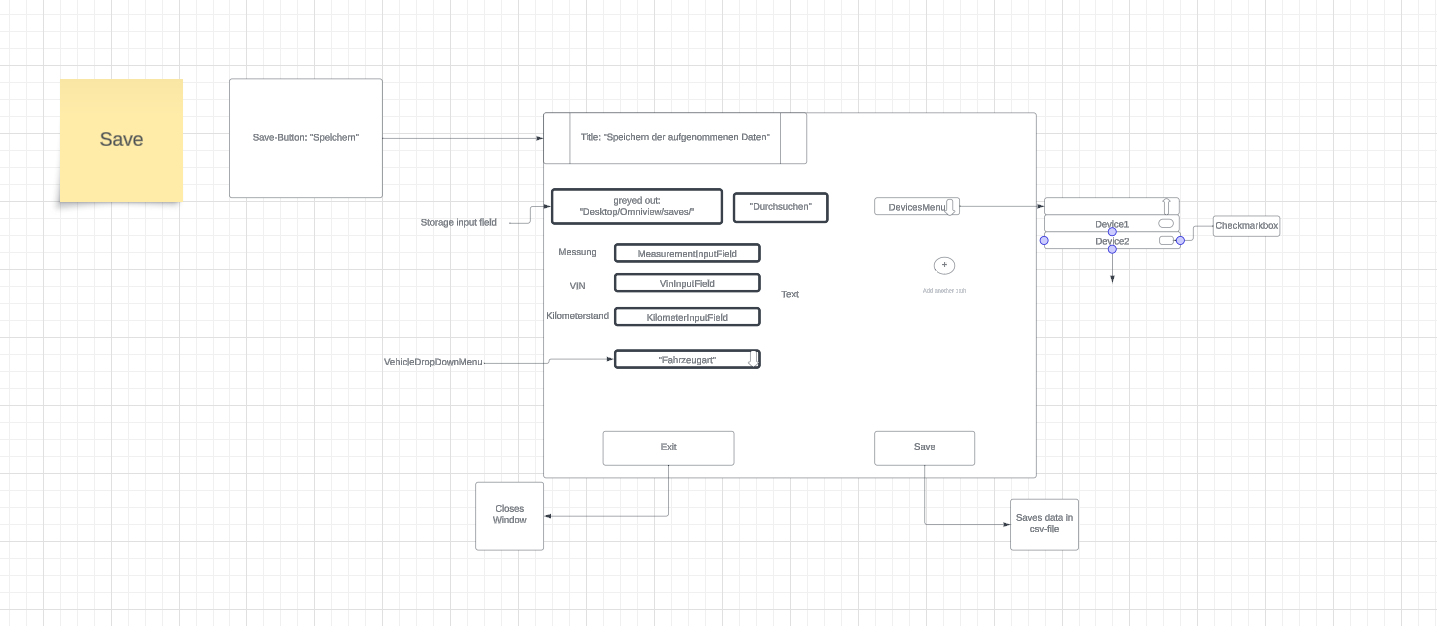
\includegraphics[width=.9\textwidth]{SaveandOpenLucidChartScreenshot.png}
    \caption[]{A visual representation of the saving process in the user interface}
    \label{fig:saveData}
\end{figure}

\subsubsection{Settings button}

\subsubsection{load again button}

\subsubsection{start and stop button states}



\subsection{Datawindow}

The following parts of the view should be adjustable: 

\begin{itemize}
    \item screensize
    \item scale of the x- and y-axis 
    \item fontsize 
\end{itemize}

The adjustments should be able to be made per mouse, mousepad, touchpad and with shortcuts. They also should be able to be set to a specific number. 
The user should be able to zoom in the dataset and cut out a specific part of the data. The image of the data should be able to be converted into a PDF. 

\subsection{Data upload window}

The upload window should be an extra window that does not overlap with the datawindow. It should contain an upload button and an exit button. The user should be able to put in the 
current dataset or another dataset from their database. 
The window should contain fields where the user can put in 
\begin{itemize}
    \item the analysis type
    \item the base data like the workplace of the measurement
    \item the reasons for the measurement
    \item if the measurement shows expected course or not 
\end{itemize}



\subsection{Help menu}

The Helpmenu should contain 
\begin{itemize}
    \item a link to our ous
    \item a link to an Tutorial website
\end{itemize}

\section{Design Principles}\label{cap:Designprinciples}
\subsection{Design of Popupwindows}\label{cap:Designprinciples_Popupwindows}
\subsubsection{Design of Buttons in PopupWindows}\label{cap:Designprinciples_PopupWindowButtons}
\subsection{Design of Icon Buttons}\label{cap:Designprinciples_IconButtons}




\chapter{The Waveform-Processing-Network}
\label{chap:WaveformProcessingNetwork}
A transducer is a directed node, and serves the function of forwarding and manipulating a value of a given waveform.
Routes are directed graphs, consisting of nodes of transducers and attributeless connections between them.
Routes can be dynamically constructed. 
The Waveform-Procesing-Network it is a global singleton static object, that gets default-constructed at the epoch-servers startup, and offers the routines .addRoute(Route\_t\&\& newRoute).
These transducer-nodes might take additional construction parameters. 
A route is to be read from right to left, since the interpretation can be ambigious reading from left to right. 
Routes can be configured via a REST-API POST method, that adds a specific route to a connection. 
\chapter[Further Devl]{Further Development of OmniView}
OmniView as it is right now has a limited shelf-life. 
The current version will be deprecated somewhere around summer of 2024.
It will be replaced by a more modular approach, that consists of two separate pieces, called OmniDaemon and OmniView 2.0.
OmniView 2.0 will be written in Angular.
OmniDaemon will still be written in C++ and use the same approach for data-acquisition. 
The interprocess-communication between the data and the view on the data will be implemented by using websockets for live-streaming, REST for settings and downloading whole files and MQTT-Publishing for sending out alarms and similar fire-and-forget messages. 


\printglossaries

\end{document}